%!Mode::"UTF-8"
\documentclass[12pt]{article}

% 页面设置
\usepackage{geometry}
\geometry{left=2.5cm, right=2.5cm, top=2.5cm, bottom=2.5cm}
\usepackage{graphicx}
\usepackage{ctex}
\usepackage{fontspec}
\usepackage{setspace}
\usepackage[version=4]{mhchem}

% 代码设置
\usepackage{listings}
\usepackage{color}
\setmonofont{Consolas}
\definecolor{listing}{gray}{0.97}
\lstset{
	backgroundcolor=\color{listing},
	basicstyle=\footnotesize,
	numbers=left,
	numberstyle=\footnotesize,
	stepnumber=1,
	aboveskip={0.5\baselineskip},
	belowskip={0.5\baselineskip},
	columns=fullflexible,
	breaklines=true,
	breakatwhitespace=true,
	frame=single,
	basicstyle=\ttfamily,
	numberstyle=\ttfamily,
	tabsize=2
}

% 字体设置
\setmainfont{Times New Roman}
\setCJKmainfont{SimSun}
\setCJKsansfont{SimHei}

% 表格设置
\usepackage{makecell}
\newcommand{\addcell}[2][4]{\makecell{\zihao{#1}\textsf{#2}}}
\usepackage{titlesec}
\usepackage{booktabs}
\usepackage{tabularx}

% 设置图注、表注
\usepackage{caption}
\usepackage{bicaption}
\captionsetup{labelsep=quad, font={small, bf}, skip=2pt}
\DeclareCaptionOption{english}[]{
    \renewcommand\figurename{Fig.}
    \renewcommand\tablename{Table}
}
\captionsetup[bi-second]{english}

% 设置页眉
\usepackage{fancyhdr}
\pagestyle{fancy}
\fancypagestyle{preContent}{
    \fancyhead[L]{\zihao{-5} 物理化学实验}
    \fancyhead[C]{\zihao{-5} 实验十三\ \ 紫外可见吸收光谱仪的搭建与量子一维势阱方程检验}
    \fancyhead[R]{\zihao{-5} 1800011828\ 王宇哲}
}
\pagestyle{preContent}

%	设置首页页眉页脚
\fancypagestyle{plain}{
	\fancyhead[L]{\zihao{-5} 物理化学实验}
	\fancyhead[C]{\zihao{-5} 实验十三\ \ 紫外可见吸收光谱仪的搭建与量子一维势阱方程检验}
	\fancyhead[R]{\zihao{-5} 1800011828\ 王宇哲}
	\cfoot{}
}

% 设置标题格式
\titleformat*{\section}{\zihao{4}\sffamily}
\titleformat*{\subsection}{\zihao{-4}\sffamily}
\titleformat*{\subsubsection}{\zihao{-4}\sffamily}
\titlespacing*{\section}{0pt}{10pt}{10pt}
\titlespacing*{\subsection}{0pt}{10pt}{5pt}
\titlespacing*{\subsubsection}{0pt}{10pt}{5pt}

% 设置引用格式
\usepackage[super,round,comma,compress]{natbib}

\usepackage{amsmath}
\usepackage{amssymb}

%设置封面
\begin{document}
    % 标题页
    \begin{titlepage}
    	% 页眉
    	\thispagestyle{plain}
        % 图片
        \begin{figure}[h]
            \centering
            \includegraphics{pku.png}
        \end{figure}
        \vspace{24pt}
        % 标题
        \centerline{\zihao{-0} \textsf{物理化学实验报告}}
        \vspace{40pt} % 空行
        \begin{center}
            \begin{tabular}{cp{13 cm}}
                % 题目
                \addcell[2]{题目:\ } & \addcell[2]{\zihao{-3} 紫外可见吸收光谱仪的搭建与量子一维势阱方程检验} \\
                \cline{2-2}
            \end{tabular}
        \end{center}
        \vspace{20pt} % 空行
        \begin{center}
            \doublespacing
            \begin{tabular}{cp{5cm}}
                % 姓名
                \addcell{姓\phantom{空格}名:\ } & \addcell{王宇哲} \\
                \cline{2-2}
                % 学号
                \addcell{学\phantom{空格}号:\ } & \addcell{1800011828}\\
                \cline{2-2}
                % 组别
                \addcell{组\phantom{空格}别:\ } & \addcell{11组} \\
                \cline{2-2}
                % 实验日期
                \addcell{实验日期:\ } & \addcell{2020.10.21及10.28}\\
                \cline{2-2}
                % 室温
                \addcell{室\phantom{空格}温:\ } & \addcell{294.35\ K}\\
                \cline{2-2}
                % 大气压强
                \addcell{大气压强:\ } & \addcell{102.73\ kPa}\\
                \cline{2-2}
            \end{tabular}
            \begin{tabular*}{\textwidth}{c}
                \\ % 这是空行
                \\ % 这是空行
                \\ % 这是空行
                \\ % 这是空行
                \hline % 分割线
            \end{tabular*}
        \end{center}
        % 摘要
        \textsf{摘\ \ 要}\ \ 本实验利用实验室提供的部件搭建了紫外可见吸收光谱仪,利用氘灯对光谱仪进行了调试和标定;用光谱仪测定了同一物质不同浓度溶液的吸收光谱,拟合工作曲线,验证了Lambert-Beer定律,并对比了使用氘灯光源和卤钨灯光源的差异;测量了多个共轭分子的吸收光谱,计算了各分子的摩尔吸光系数$\varepsilon$;分别用一维势阱模型和Gaussian程序对各分子进行了模拟计算,比较了计算结果与实验结果的差别。
        \\
        \\
        % 关键字
        \textsf{关键词}\ \ 紫外可见吸收光谱仪;一维势阱模型;Lambert-Beer定律;Gaussian程序
    \end{titlepage}

    \section{引言}
	略
               
\vbox{}        
    \section{实验部分}
    	\subsection{仪器和药品}
    	\subsubsection{光谱仪部件}
    	光源,光阑,平凸透镜(2个),样品池架,样品池(2个),狭缝,凹面镜(2个),光栅,ccd检测器,光学平台(面包板),光学元件架,光学支杆套件,遮光器材,安装工具。
    	\subsubsection{试剂}
    	6种共轭分子的乙醇溶液,乙醇。\par
    	6种共轭分子$\rm{(A)}\sim\rm{(F)}$的结构如\textbf{图1}所示。
    	 \begin{figure}[h]
    		\centering
    		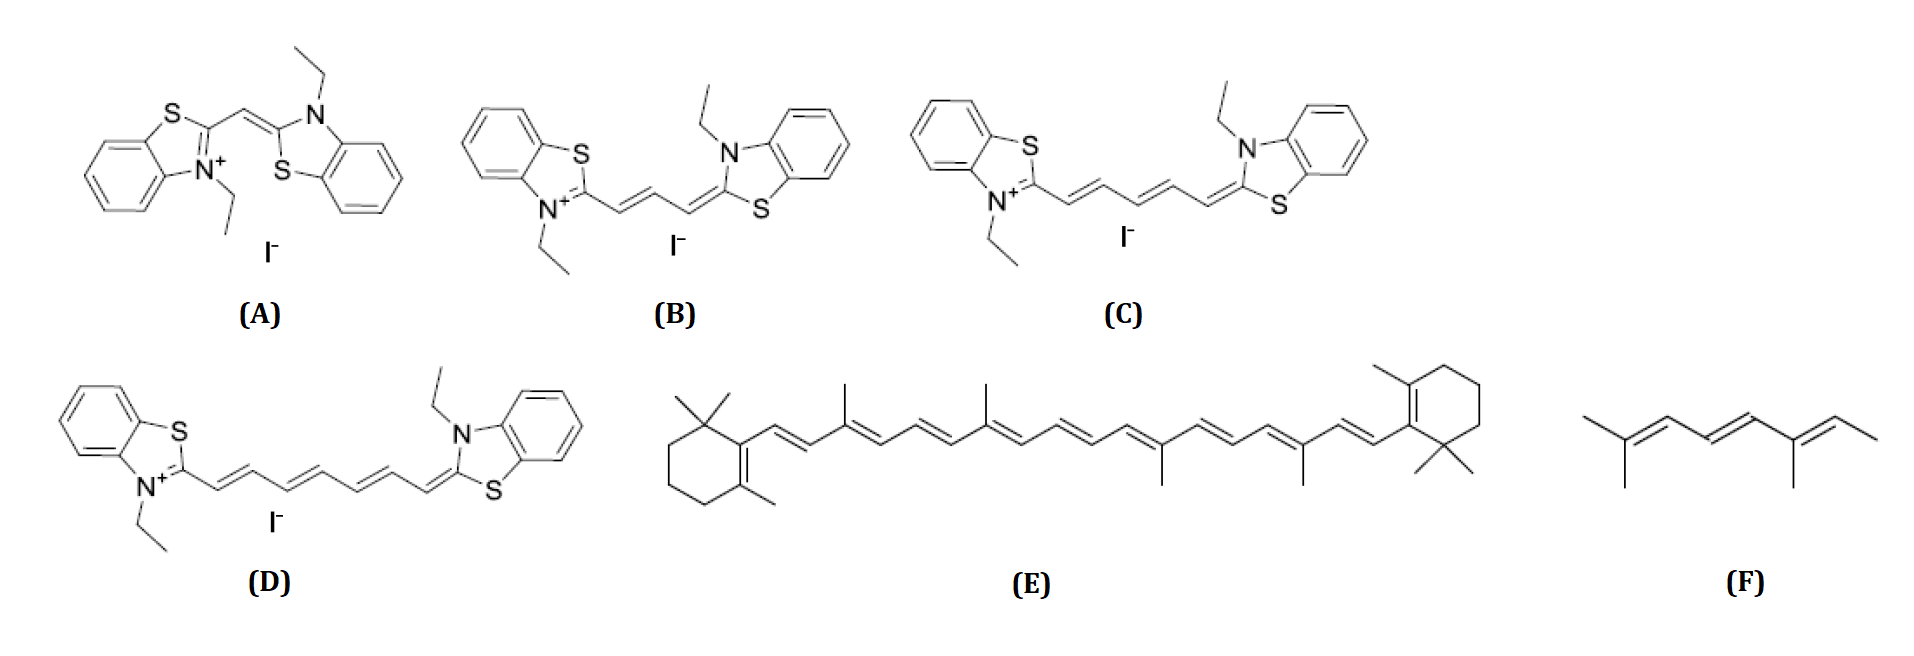
\includegraphics[width=1\textwidth]{1.png}
    		\bicaption{6种共轭分子的结构}{Structures of 6 conjugated molecules}
    	\end{figure}
    	\par
    	
    	
    	 \subsection{实验内容\citealp{physchemlab}}
			\subsubsection{紫外可见光谱仪的搭建}
		将各个光学元件固定在元件架中,放回到光学支杆套杆上。\par
		打开氘灯电源,将凸透镜套组固定在光源左侧约$75{\rm\ \ mm}$处,调整凸透镜高度,使透射光成为平行光;在凸透镜后适当位置固定样品池架,在光源和凸透镜之间安装光阑,使样品池获得合适的光斑;在样品池后适当位置安装第二个凸透镜套组,使光束形成会聚光,将可调狭缝固定于此处;打开卤钨灯,使得光斑最小且通过狭缝。\par
		在狭缝后顺光方向约$100{\rm\ \ mm}$处固定第一个凹面镜套组,使反射光与入射光成一尽量小的夹角,且反射光近似于平行光;沿反射光方向合适位置安装光栅套组,令光照在光栅的正中;反复调节光栅与入射光之间的夹角,用实验室提供的白纸板观察分光方向,直至得到较强的一级衍射。\par
		在光栅的一级衍射方向上固定第二个凹面镜套组,用白纸板确定反射光焦点位置,将ccd固定在此处;调整光栅与第二个凹面镜的距离,使凹面镜和ccd尽量接收到全部光谱范围($200\sim800 \ \ {\rm nm}$,即红光至蓝光占受光面积的$3/5$)。\par
		用实验室提供的纸板将狭缝及之后的光路仔细遮光,并在狭缝前的纸板上开一小孔,以便光线射入;再用纸板和遮光布将光谱仪罩好。
			\subsubsection{光谱仪的标定}
		打开氘灯光源,打开电脑,连接好ccd,运行ccd控制软件,扫描光源谱图,在线调整光栅之后光路,对ccd的位置进行微调,观察分辨率的改善;观察到各特征峰足够明显时,彻底固定光栅之后光路和ccd的位置,找到氘灯各个特征峰。\par
		利用氘灯3个特征峰对应的ccd像素值,作图拟合得到光谱仪的$\lambda-$pixel关系,从而对光谱仪进行标定。
		
			\subsubsection{不同吸光度溶液、不同光源下的吸收光谱}
			配制$\rm{(C})$分子不同浓度的乙醇溶液,使吸光度约为$2.0,\ \  1.0,\ \ 0.5,\ \ 0.1, \ \ 0.05$;只开卤钨灯,将卤钨灯光源稳定半小时,调整积分时间为$100 \ \ {\rm ms}$以获得足够的信号强度;采集并扣除暗背景信号,保存各个样品及空白溶剂的光谱数据;观察不同吸光度下谱图的区别;\par
			配制$\rm{(C})$分子吸光度约为0.5的溶液,只开卤钨灯,测量吸收光谱;调整积分时间,同时打开卤钨灯和氘灯,再测量吸收光谱;比较两种光源所得谱图的区别。
 	\subsubsection{测定各共轭分子的吸收光谱}
 	配制其他各共轭分子的乙醇溶液,打开适当光源,测定各分子的紫外可见吸收光谱,记录室温为$294.35 \ \ {\rm K}$,样品池厚度为$10 \ \ {\rm mm}$。

 \section{数据与结果}
 \subsection{实验数据记录及处理}
 \subsubsection{光谱仪的标定}
 用氘灯对光谱仪进行标定;调整积分时间为$15\ \ {\rm ms}$,扫描得到氘灯的发射谱图如\textbf{图2}所示。从\textbf{图2}中可以看出,氘灯发射光谱有三个明显的特征峰,对照氘灯的参考发射光谱图,可知从左至右三个特征峰标准谱线的波长分别为$\lambda=656.06\ \ {\rm nm}$、$\lambda=581.39\ \ {\rm nm}$、$\lambda=485.82\ \ {\rm nm}$,即低pixel处对应较长波长。
  \begin{figure}[h]
 	\centering
 	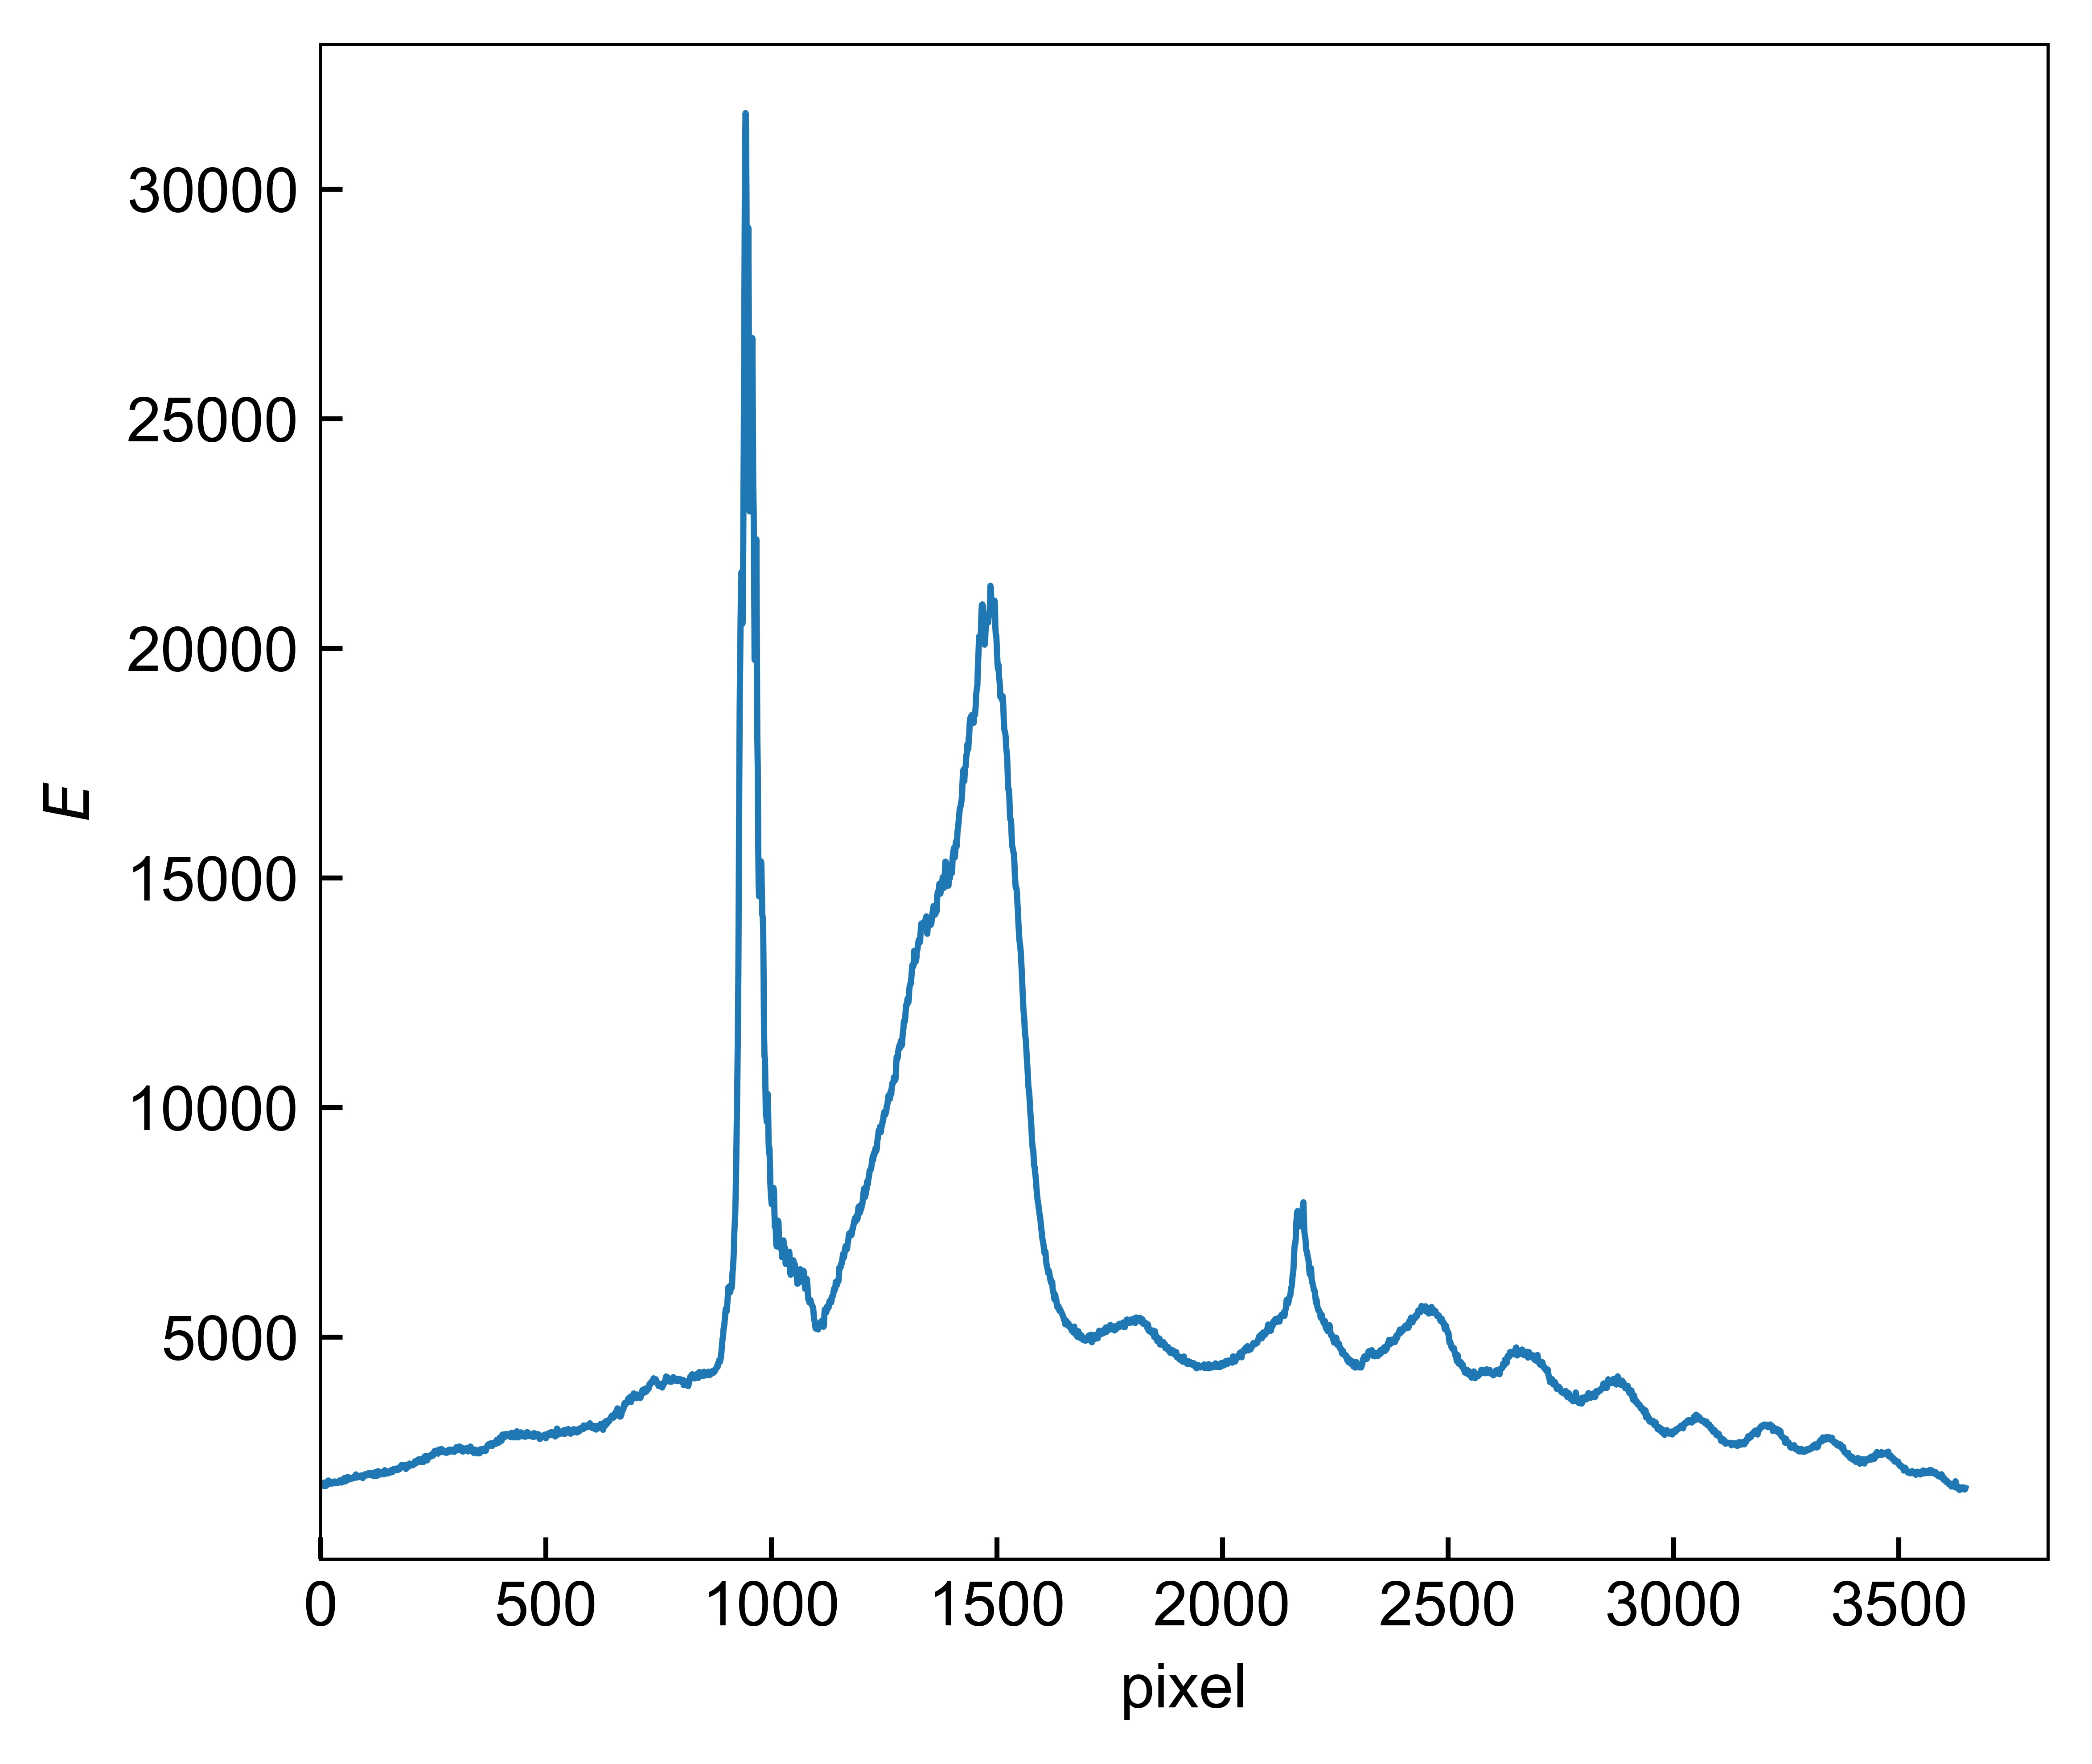
\includegraphics[width=0.6\textwidth]{2.jpg}
 	\bicaption{实验扫描氘灯发射谱图}{Experimental deuterium lamp emission spectrum}
 \end{figure}
\par
找出三个特征峰所对应的pixel位置;各特征峰标准谱线波长$\lambda$及对应的pixel位置示于\textbf{表1}。
\begin{table}[h]
	\centering
	\zihao{5}
	\bicaption{光谱仪$\lambda$-pixel数据}{Spectrometer $\lambda$-pixel data}
	\begin{tabular}{ccc}
		\toprule
		序号 & $\lambda/{\rm nm}$ & pixel  \\
		\midrule
		1 & 656.06 & 943 \\
		2 & 581.39 & 1486 \\
		3 & 485.82 & 2180 \\
		\bottomrule
	\end{tabular}
\end{table}
\par
利用\textbf{表1}数据作散点图如\textbf{图3}所示,可见各点近似落在一条直线上;对$\lambda$-pixel进行线性拟合,所得回归直线也示于\textbf{图3}中。拟合得到的回归直线表达式为
$$\lambda / {\rm nm}=-0.1376 \ \ pixel +785.86,\ \ R=0.99999992
$$
\par
读取ccd像素范围为$0\sim3648$,故代入拟合直线方程,计算得到光谱仪可测波长范围为$283.80\ \ {\rm nm} \sim 785.86\ \ {\rm nm}$。

\vbox{}

\vbox{}

\begin{figure}[h]
	\centering
	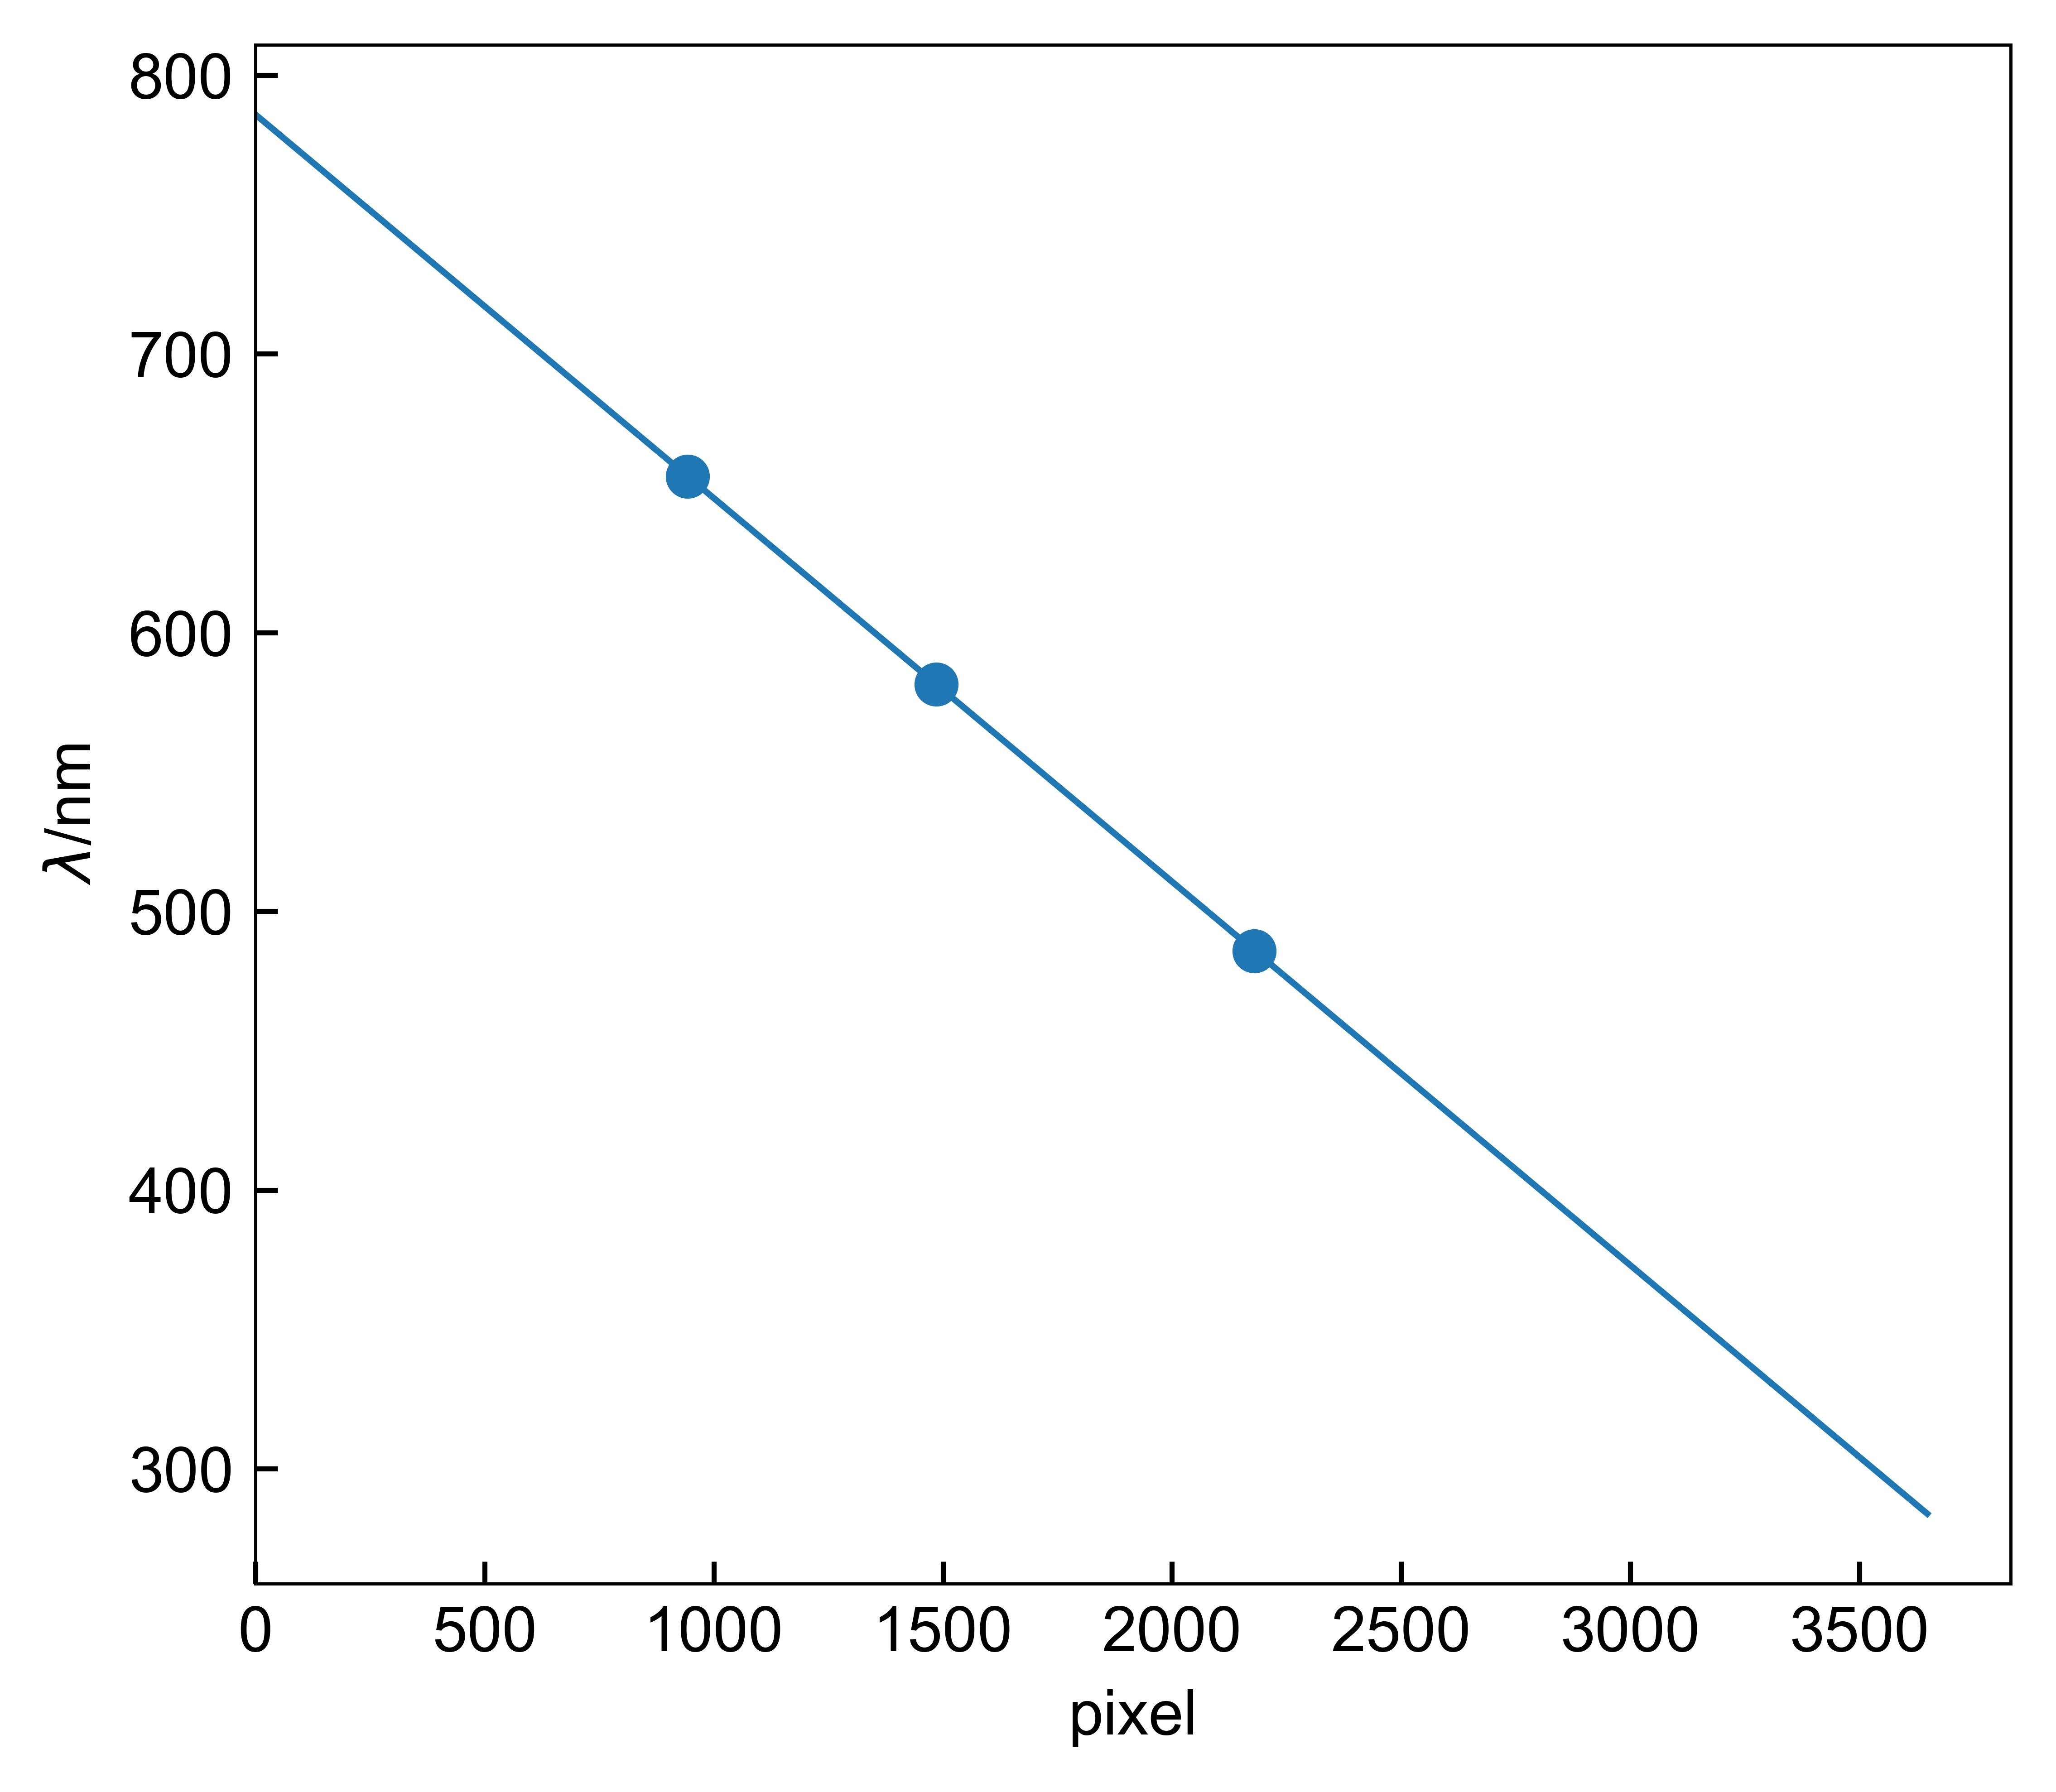
\includegraphics[width=0.6\textwidth]{3.jpg}
	\bicaption{$\lambda$-pixel关系图}{Correlation of $\lambda$-pixel}
\end{figure}
\par




 \subsubsection{不同吸光度溶液的吸收光谱}
 将$20\ \ \mu{\rm M}$的${\rm(C)}$的乙醇溶液进行稀释,得到三组不同浓度的溶液;溶液配制过程中所取原溶液浓度$c_{0}$、体积$V_{0}$、加入乙醇体积$V_{EtOH}$、所得溶液浓度$c$示于\textbf{表2}。
 \begin{table}[h]
 	\centering
 	\zihao{5}
 	\bicaption{$\rm(C)$溶液的配制}{$\rm(C)$ solution preparation}
 	\begin{tabular}{ccccc}
 		\toprule
 		序号 & $c_{0}/\mu{\rm M}$ & $V_{0}/{\rm mL}$ & $V_{EtOH}/{\rm mL}$ & $c/\mu{\rm M}$  \\
 		\midrule
 		1 & 20 & 5 & 0 & 20 \\
 		2 & 20 & 3 & 3 & 10 \\
 		3 & 20 & 1 & 4 & 4 \\
 		\bottomrule
 	\end{tabular}
 \end{table}
 \par
 只开卤钨灯,设定积分时间$1\ \ {\rm s}$,采集并扣除暗背景信号,保存各个样品的透过光强$I$及空白溶剂的透过光强$I_{0}$,利用公式
 $$
 A=lg(\frac{I_{0}}{I})
 $$
 计算吸光度$A$与波长$\lambda$的关系,结果示于\textbf{图4}。可以看出,三条曲线的主吸收峰位置比较接近,均位于$649.0\ \ {\rm nm}$附近。
 \begin{figure}[h]
 	\centering
 	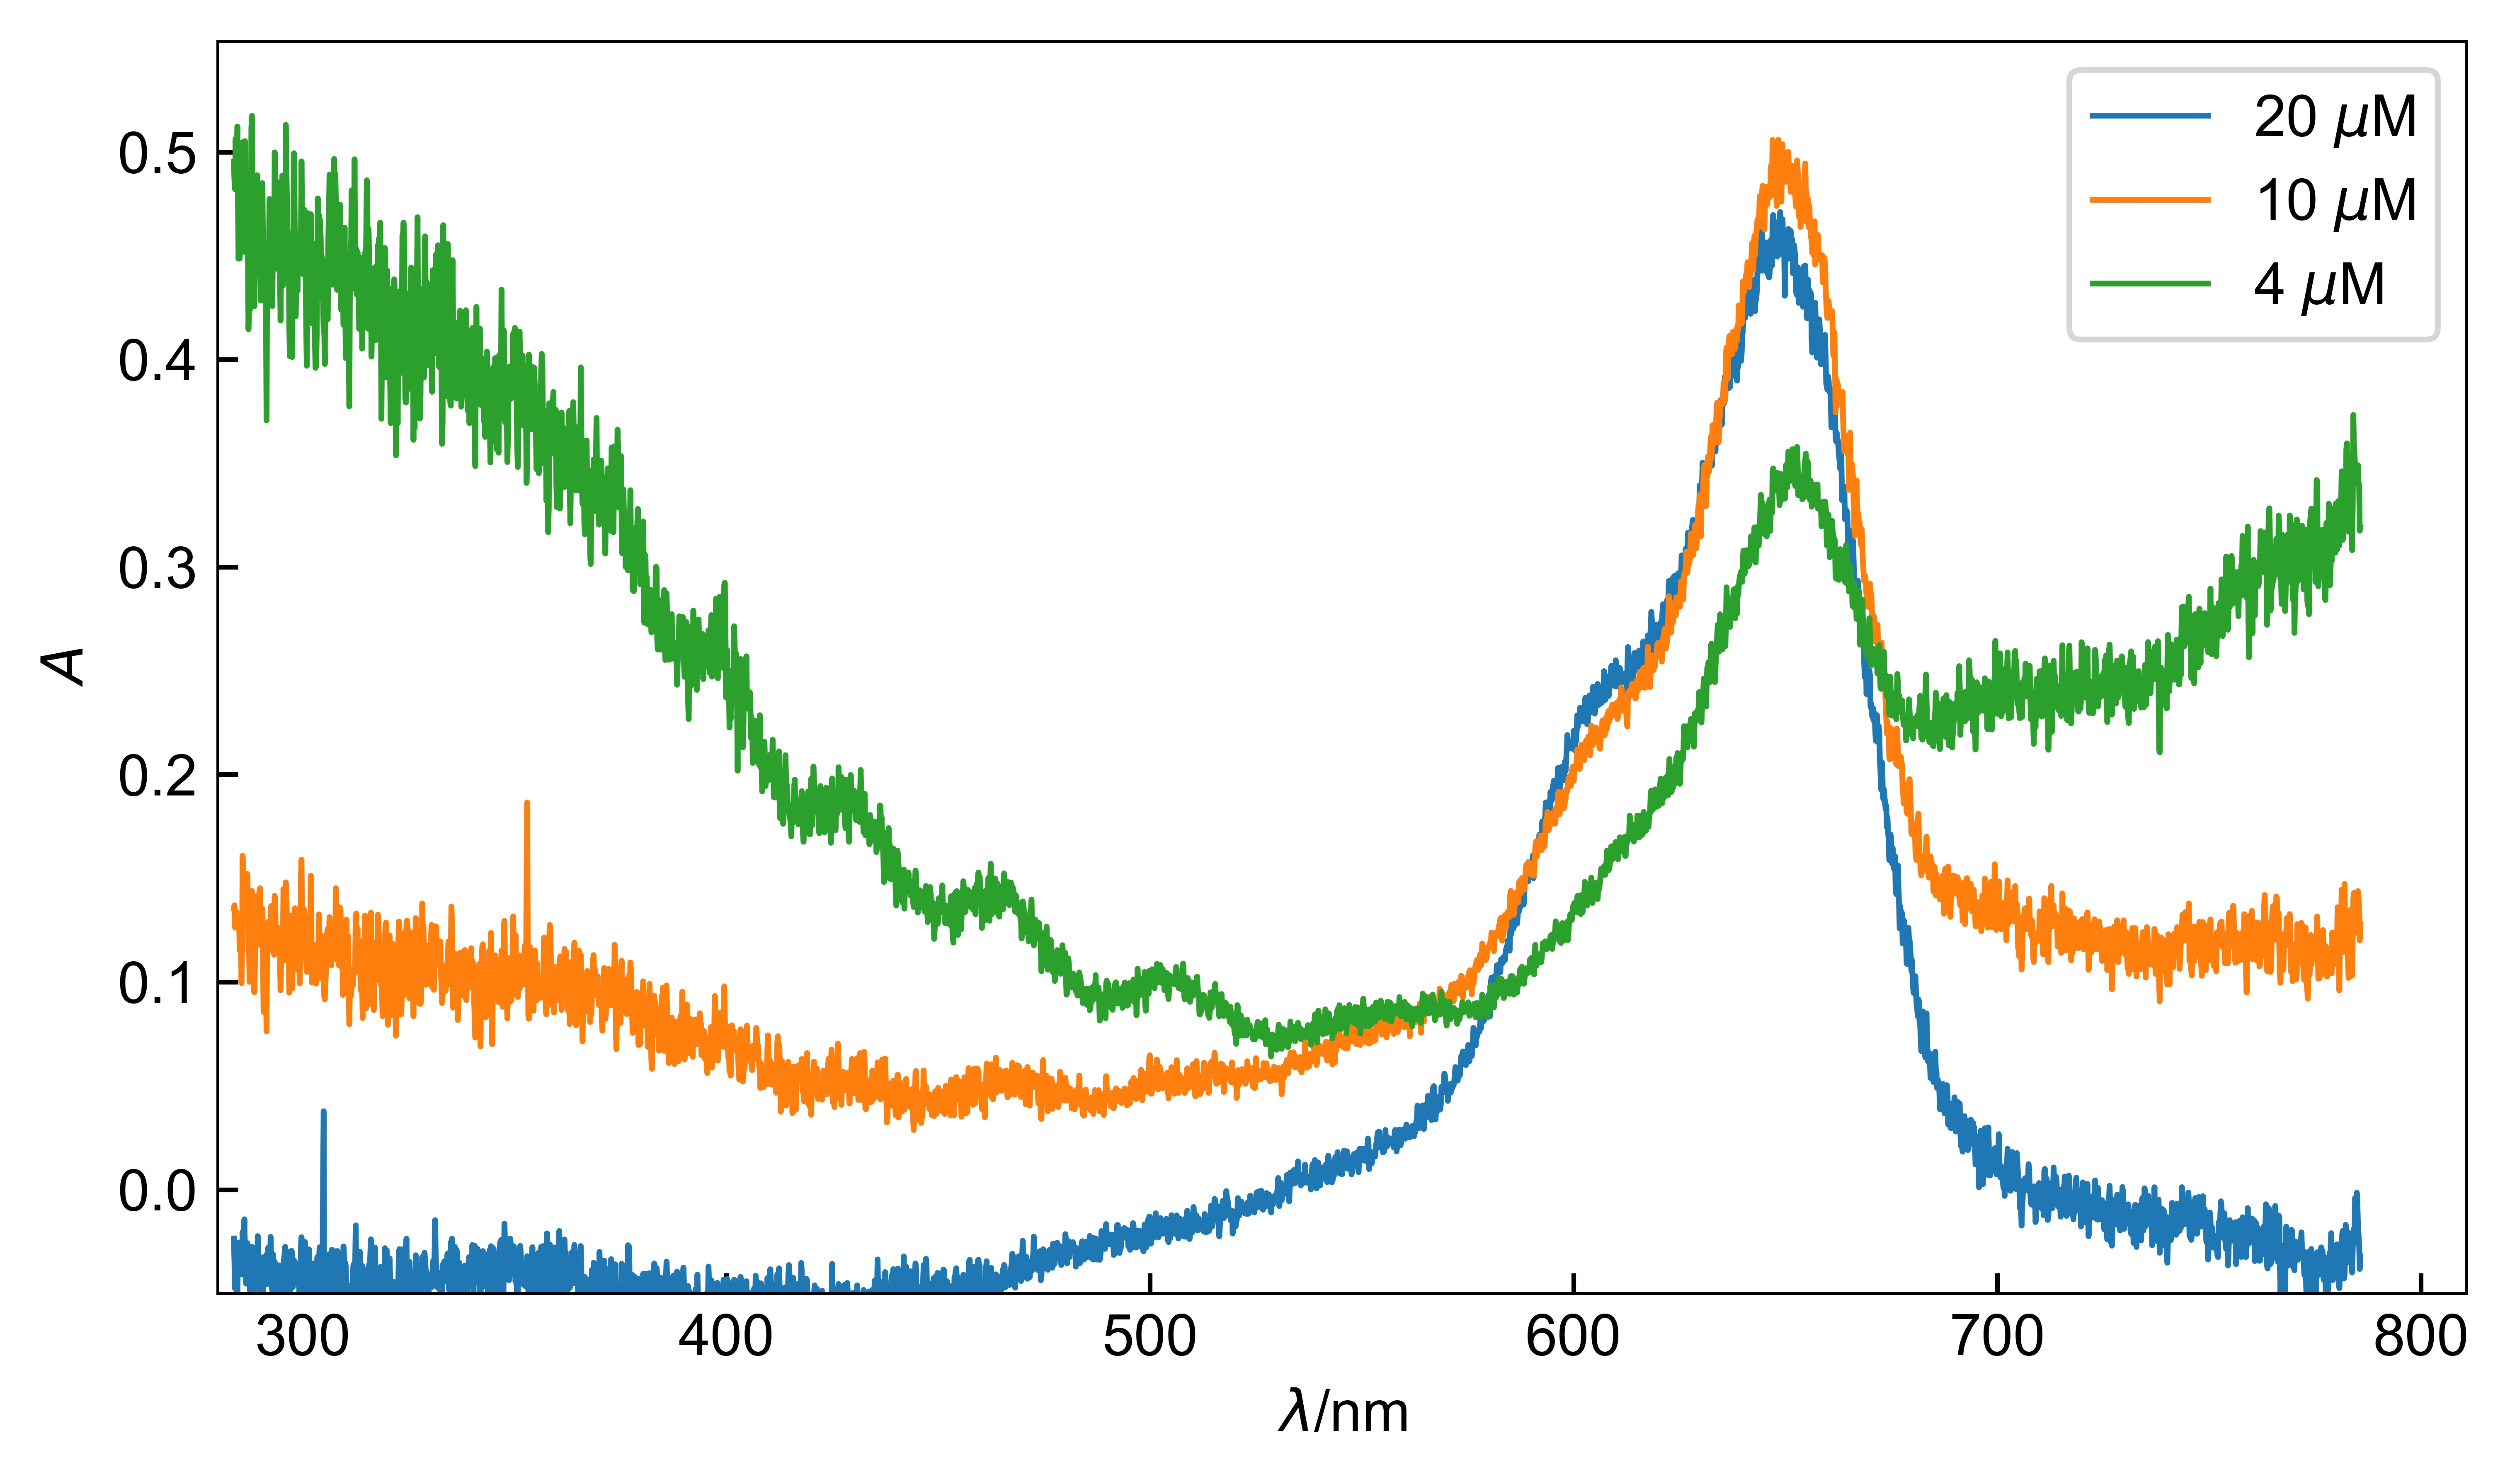
\includegraphics[width=0.8\textwidth]{4.jpg}
 	\bicaption{不同吸光度溶液的吸收光谱}{Absorption spectra of solutions with different absorbance}
 \end{figure}
 \par
 根据\textbf{图4},可见本次实验所搭建的光谱仪在进行不同吸光度溶液的光谱测定时出现了严重的问题,具体而言有以下两点:其一是信噪比低,噪声导致的曲线波动极大,且在实际实验中无法通过简单地改变积分时间或对输出取平均值进行有效改善(实际实验中两种方法均进行了尝试,但都未收到很好的效果);其二是在$\lambda_{max}$波段的定量测量仍然有相当可观的误差,导致吸光度$A$与溶液浓度$c$未能呈现出很好的线性关系,甚至未能呈现出单调关系。\par
 究其原因,可能是因为以下两点:其一,在搭建光谱仪时光路存在一定问题,导致光线发散或不准直,从而使得样品池中待测溶液吸光效果较差;从\textbf{图4}可以看出,对于${\rm (C)}$,即使取未加稀释的、浓度为$20\ \ \mu {\rm M}$的原溶液进行测量,在$\lambda_{max}$下的吸光度$A$也不足0.5,导致低浓度溶液的吸光度测量出现很大误差;其二,在实验过程中,由于时间紧张及操作失误,没有在每次测量溶液吸收光谱前重测乙醇溶液的吸光度,而是使用同一份乙醇溶液的吸收光谱作为参比,从而导致了较大误差。\par 
 从\textbf{图4}中可以看出,不同浓度的${\rm (C)}$溶液信噪比也不同,浓度较高的$20\ \ \mu{\rm M}$溶液相对而言曲线较为光滑,信号比较明显,吸光度曲线合理;而$10\ \ \mu{\rm M}$和$4\ \ \mu{\rm M}$在波长$\lambda$较大或较小时均出现了不合理的吸光度值。因此实际测量${\rm (C)}$分子的吸收光谱时,使用$20\ \ \mu{\rm M}$的${\rm (C)}$溶液进行测定。
 \subsubsection{不同光源下的吸收光谱}
 在实验测定同种物质不同光源下的吸收光谱时,由于实际的时间安排问题,测量$\rm (C)$溶液在氘灯+卤钨灯混合光源下的吸收光谱时,${\rm (C)}$的乙醇溶液已经用尽;因此,改用浓度为$20\ \ \mu {\rm M}$的${\rm (A)}$溶液进行测定,以探究${\rm (A)}$物质在不同光源下吸收光谱的差异。\par 
 只开卤钨灯,设定积分时间为$1 {\rm s}$,测定溶液吸光度曲线;再同时打开氘灯和卤钨灯,设定积分时间为$100 {\rm ms}$,再次测定溶液吸光度曲线,对比示于\textbf{图5}中。
 \begin{figure}[h]
 	\centering
 	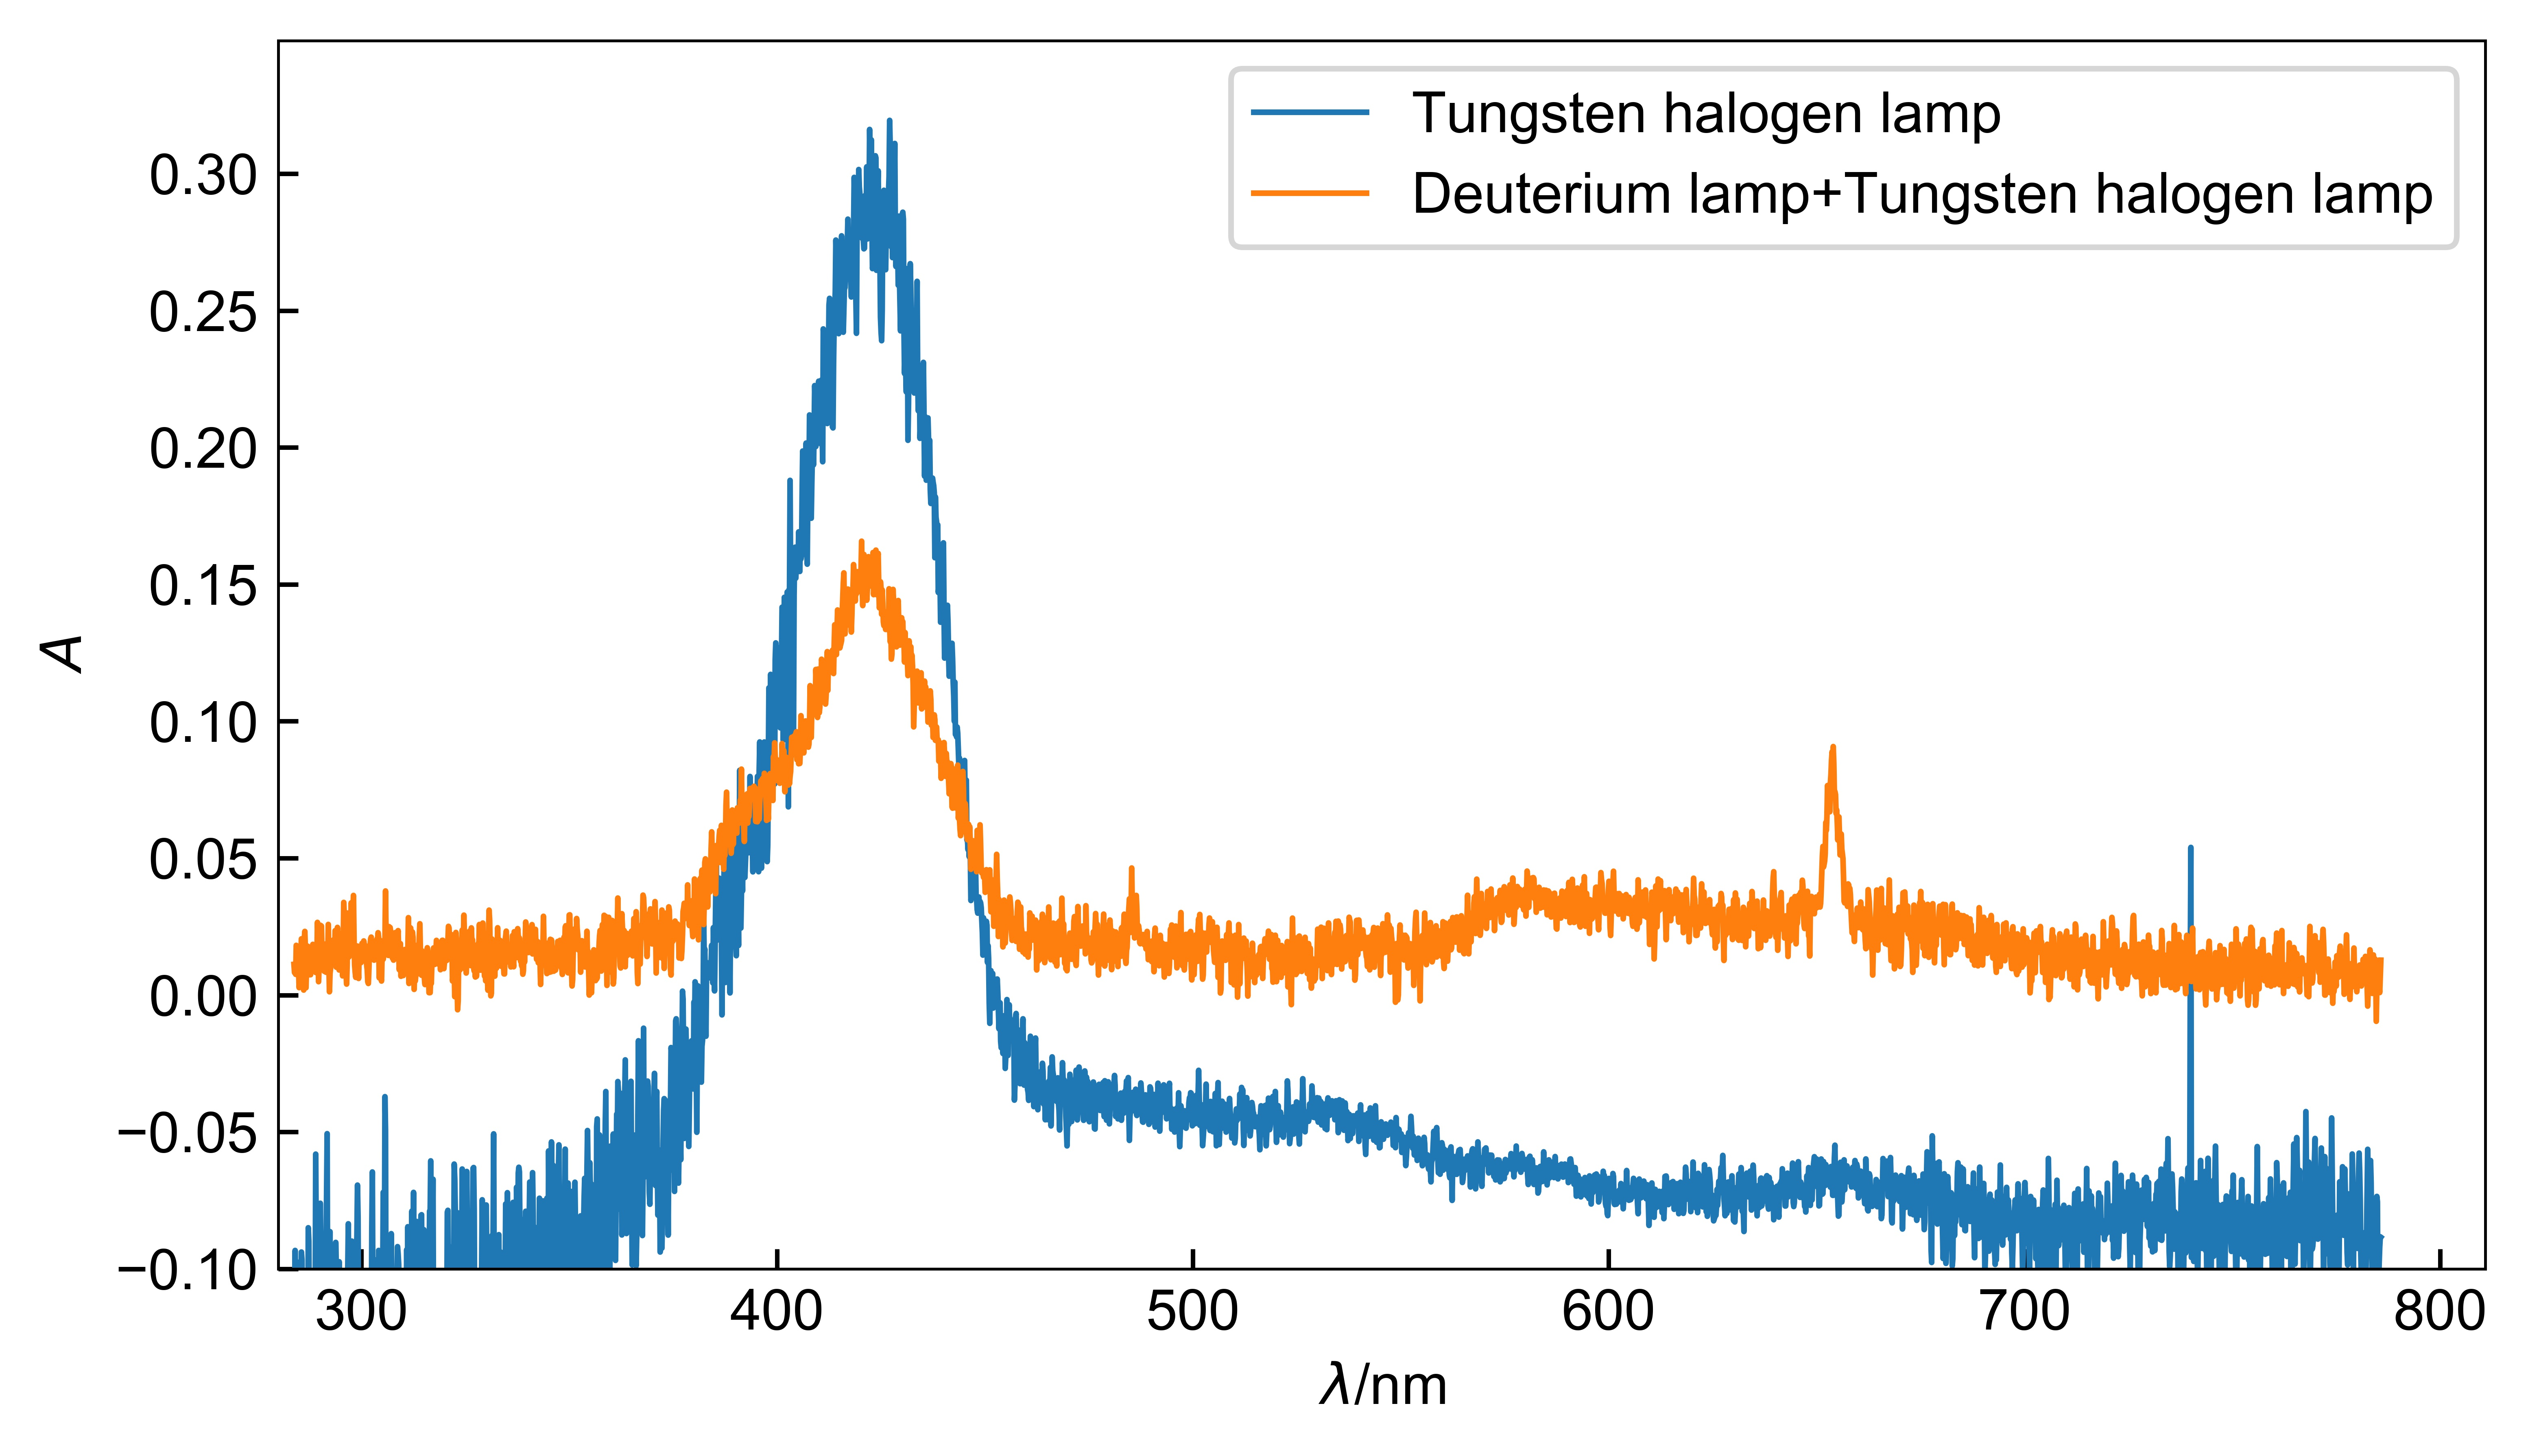
\includegraphics[width=0.8\textwidth]{5.jpg}
 	\bicaption{不同光源下$\rm (A)$溶液的吸收光谱}{Absorption spectrum of (A) solution under different light sources}
\end{figure}
\par 
根据\textbf{图5}可以看出,使用卤钨灯光源在$\lambda_{max}$处达到了更大的吸光度$A$,但使用氘灯+卤钨灯光源时吸光度曲线更平滑,信噪比更低,并且基线在0.00附近,相比单使用卤钨灯光源得到了更合理的结果。在\textbf{图5}中,使用卤钨灯光源和使用氘灯+卤钨灯光源下两条曲线在$\lambda_{max}$处达到了不同的吸光度$A$值,该现象是令人费解的,考虑到Lambert-Beer定律
$$ A=\varepsilon bc $$
表明吸光度与光源类型无关;考虑到单使用卤钨灯时,曲线有着剧烈波动,并且基线并不为0,或可以解释为该测量数据有较大误差,而使用卤钨灯+氘灯混合光源进行测量时的结果是更为准确的。这是可以理解的,因为在光路搭建的过程中主要考虑了氘灯光路,使得氘灯光源强度较高,所需积分时间更短,可以获得更优的信噪比和更好的数据可信度。\par 
可以合理推测仅使用卤钨灯和使用卤钨灯+氘灯混合光源时,测量${\rm (C)}$吸收光谱的结果。由于${\rm (C)}$的$\lambda_{max}$在$649.0\ \ {\rm nm}$附近,与氘灯$656.06\ \ {\rm nm}$处的特征峰非常接近,因此使用卤钨灯+氘灯混合光源时,在$\lambda_{max}$处将出现非常尖锐的吸收峰;而与对${\rm (A)}$的分析类似地,卤钨灯信噪比明显低于卤钨灯+氘灯混合光源。因此,对于${\rm (C)}$而言,使用卤钨灯+氘灯混合光源将大大提升吸收光谱测量的准确度和信噪比。
 
 \subsubsection{测定各共轭分子的吸收光谱}
考虑到光谱仪实际情况,直接取$\rm (A)\sim(F)$分子的原溶液测定吸收光谱。所用的各共轭分子溶液浓度如\textbf{表3}所示。\par 
 \begin{table}[h]
	\centering
	\zihao{5}
	\bicaption{各共轭分子溶液的浓度}{Concentration of each conjugated molecule solution}
\begin{tabular}{ccccc}
	\toprule
	分子 & $c_{0}/\mu{\rm M}$ & $V_{0}/{\rm mL}$ & $V_{EtOH}/{\rm mL}$ & $c/\mu{\rm M}$  \\
	\midrule
	(A) & 10 & 5 & 0 & 10 \\
	(B) & 5 & 5 & 0 & 5 \\
	(C) & 20 & 5 & 0 & 20 \\
	(D) & 3 & 5 & 0 & 3 \\
	(E) & 20 & 5 & 0 & 20 \\
	(F) & 10 & 5 & 0 & 10 \\
	\bottomrule
\end{tabular}
\end{table}
\par
根据各共轭分子溶液的颜色大致估测各自$\lambda_{max}$范围,依此在测定吸收光谱的过程中,$\rm (C)$、$\rm (D)$分子使用卤钨灯光源进行测定,积分时间$1 {\rm s}$,而$\rm (A)$、$\rm (B)$、$\rm (E)$、$\rm (F)$四个分子使用卤钨灯+氘灯混合光源进行测定,积分时间$100 {\rm ms}$。把6个分子的吸光度曲线绘制在同一张图上,用python matplotlib的自动寻峰功能,把$\lambda_{max}$位置和对应的最大吸光度$A$标注在图上,$\lambda_{max}$和$A$均取4位有效数字,如\textbf{图6}所示。
 \begin{figure}[h]
	\centering
	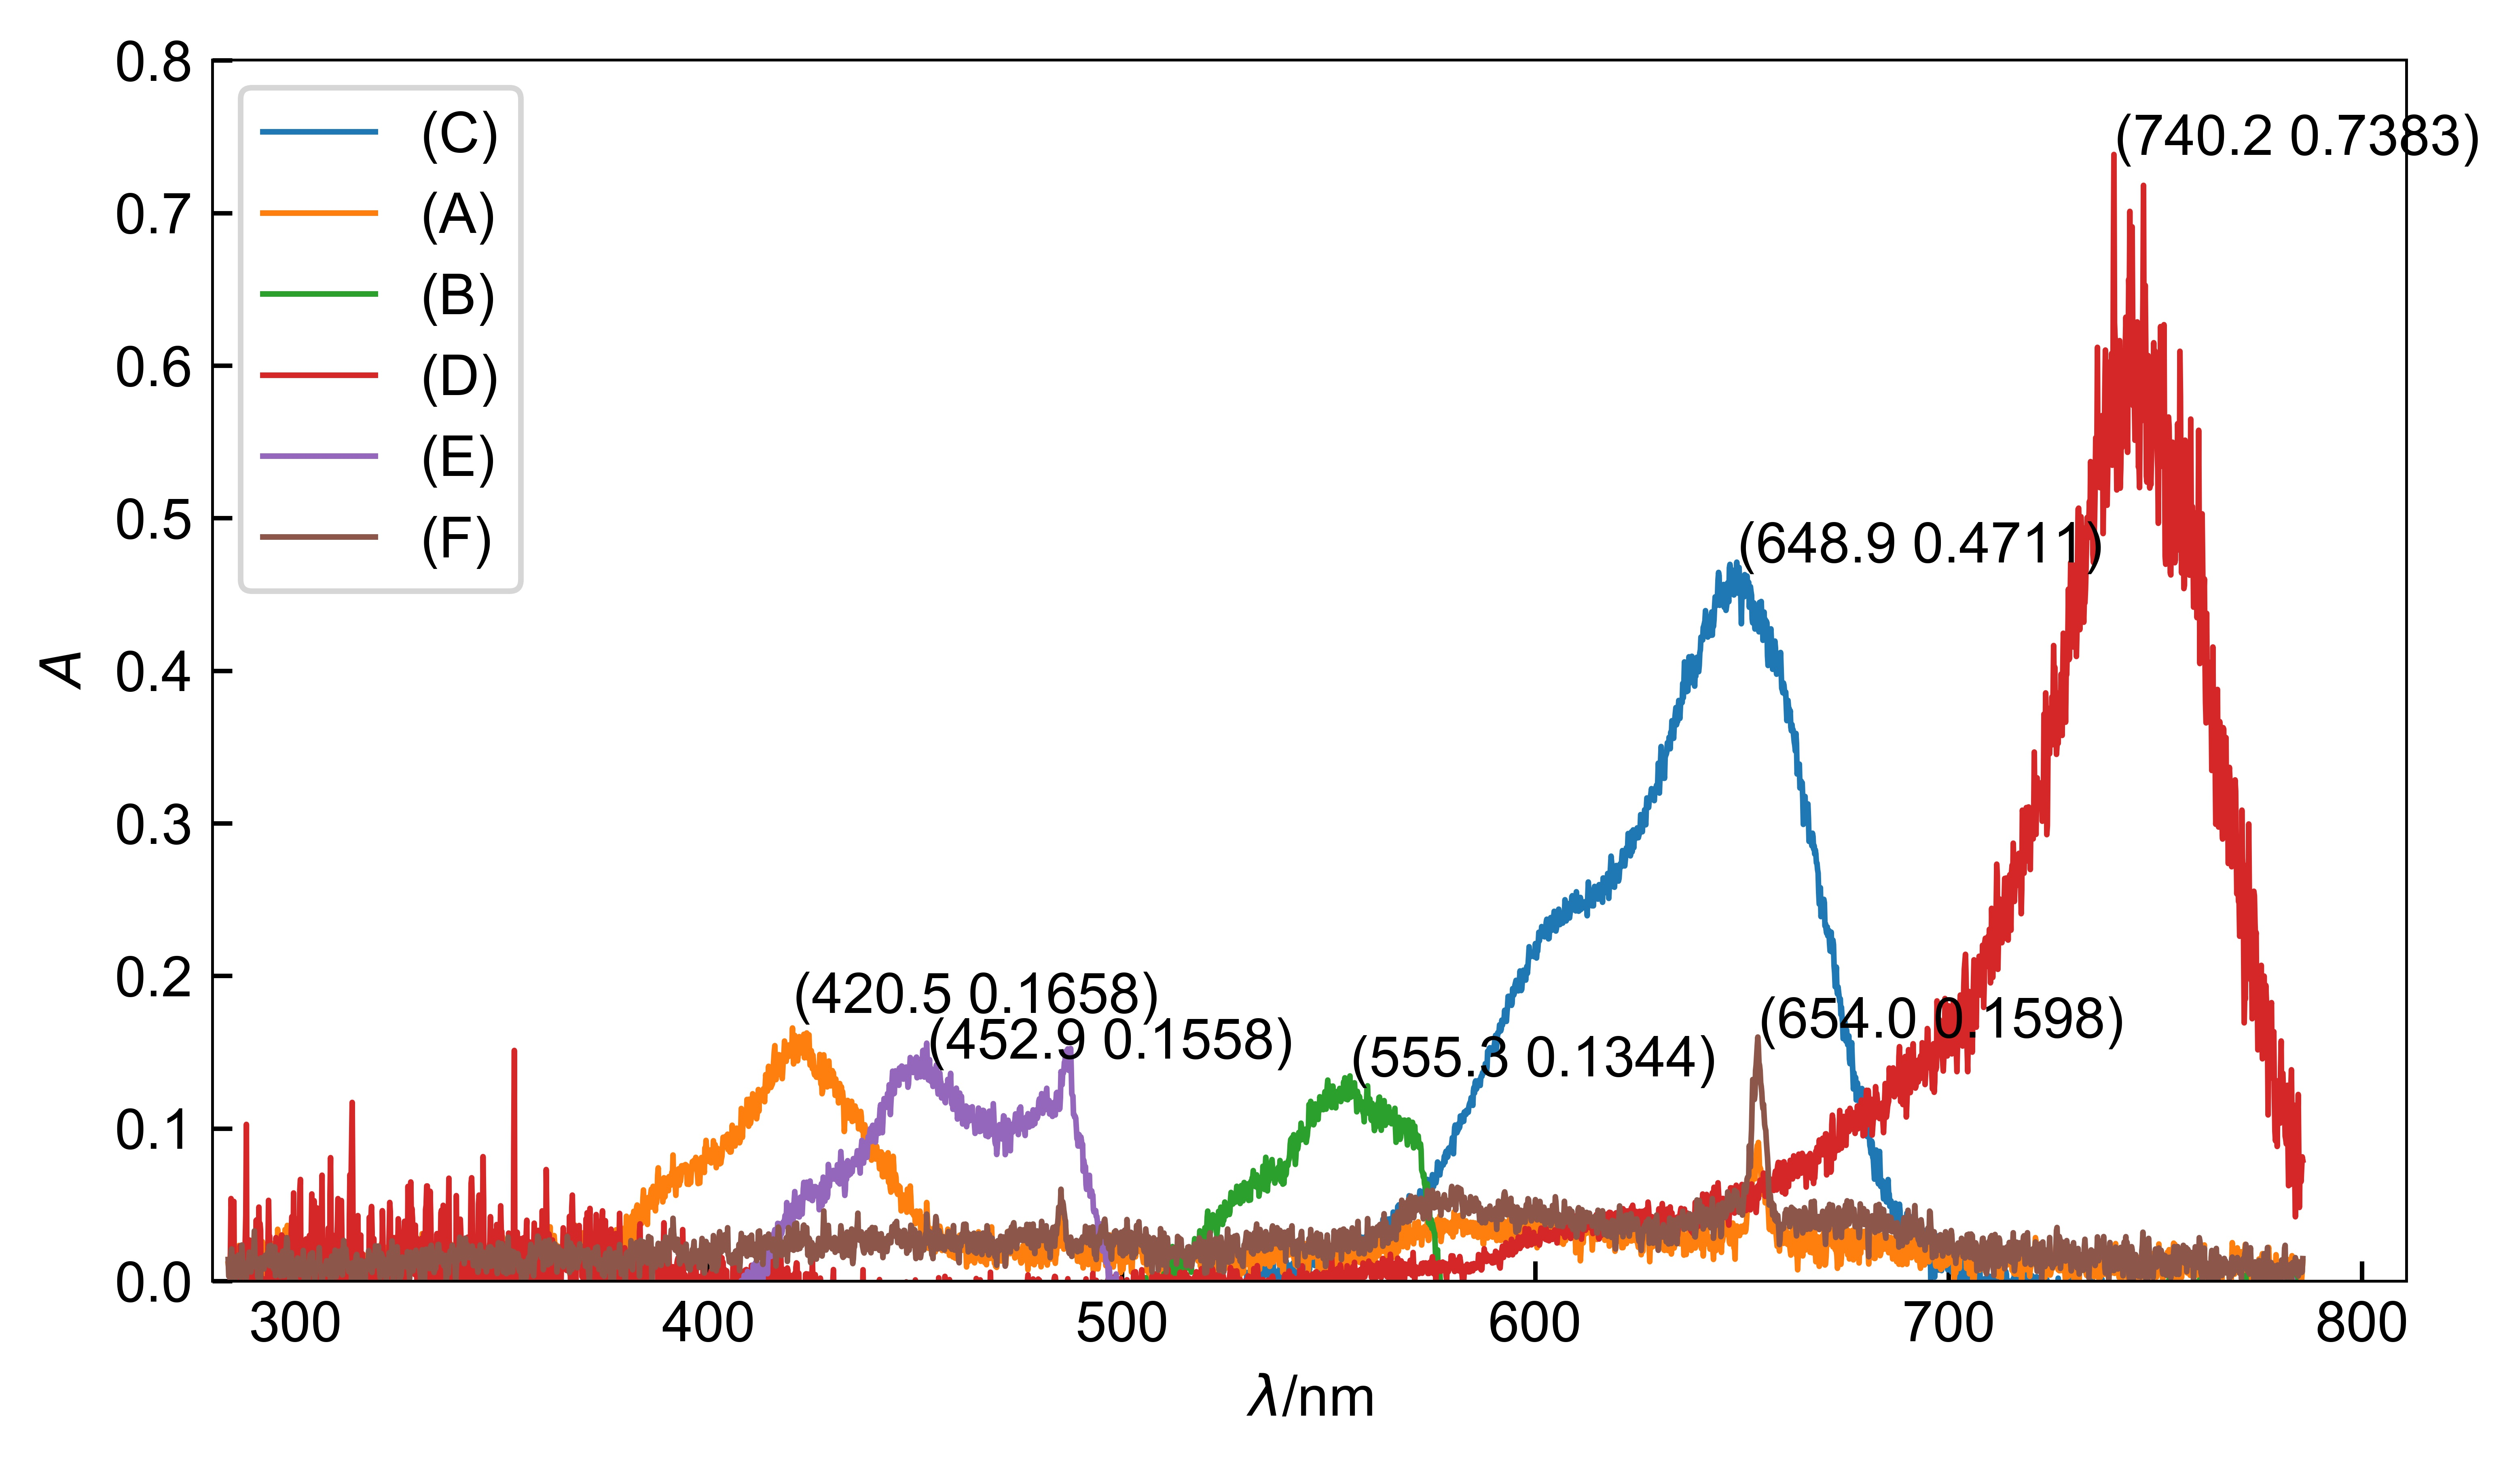
\includegraphics[width=1\textwidth]{6.jpg}
	\bicaption{各共轭分子的吸收光谱}{Absorption spectrum of each conjugated molecule}
\end{figure}
\par 
从\textbf{图6}中辨认各共轭分子的最大吸收峰,可以发现${\rm (F)}$分子标注的最大吸收位置并非实际的最大吸收峰,应当只是噪音造成的信号偏差;除此之外,其他5个分子的最大吸收峰均真实有效。测得的5个分子的最大吸收峰位置$\lambda_{max}$及对应的最大吸光度$A$列表示于\textbf{表4}中,根据Lambert-Beer定律,
$$
A=lg\frac{I_{0}}{I}=\varepsilon bc
$$
取样品池光程$b=10\ \ {\rm mm}$,计算各样品的摩尔消光系数
$$\varepsilon=\frac{A}{bc}
$$也示于\textbf{表4}中。

\begin{table}[h]
	\centering
	\zihao{5}
	\bicaption{各共轭分子的最大吸收波长$\lambda_{max}$和摩尔吸光系数$\varepsilon$}{$\lambda_{max}$ and $\varepsilon$ of each conjugated molecule}
	\begin{tabular}{ccccc}
		\toprule
		分子 & $c/\mu{\rm M}$ & $\lambda_{max}$ & $A$ & $\varepsilon/{\rm \ \ M^{-1}\cdot m^{-1}}$  \\
		\midrule
		(A) & 10 & 420.5 & 0.1658 & 1.66$\times 10^{6}$ \\
		(B) & 5 & 555.3 & 0.1344 & 2.69$\times 10^{6}$ \\
		(C) & 20 & 648.9 & 0.4711 & 2.36$\times 10^{6}$ \\
		(D) & 3 & 740.2 & 0.7383 & 2.46$\times 10^{7}$ \\
		(E) & 20 & 452.9 & 0.1558 & 7.79$\times 10^{5}$ \\
		\bottomrule
	\end{tabular}
\end{table}
\par

\subsection{计算与结果分析}
\subsubsection{Gaussian理论计算}
使用GaussView软件搭建$\rm (A)\sim (F)$6个分子,先对分子进行结构优化,将优化后的分子结构作为输入,使用PBE1PBE/6-311g(2d,p)对6个分子进行tddft激发能计算\citealp{ljr};使用GaussView打开结果文件,在Results/UV-Vis中查看结果图谱,如\textbf{图7}所示。
 \begin{figure}[h]
	\centering
	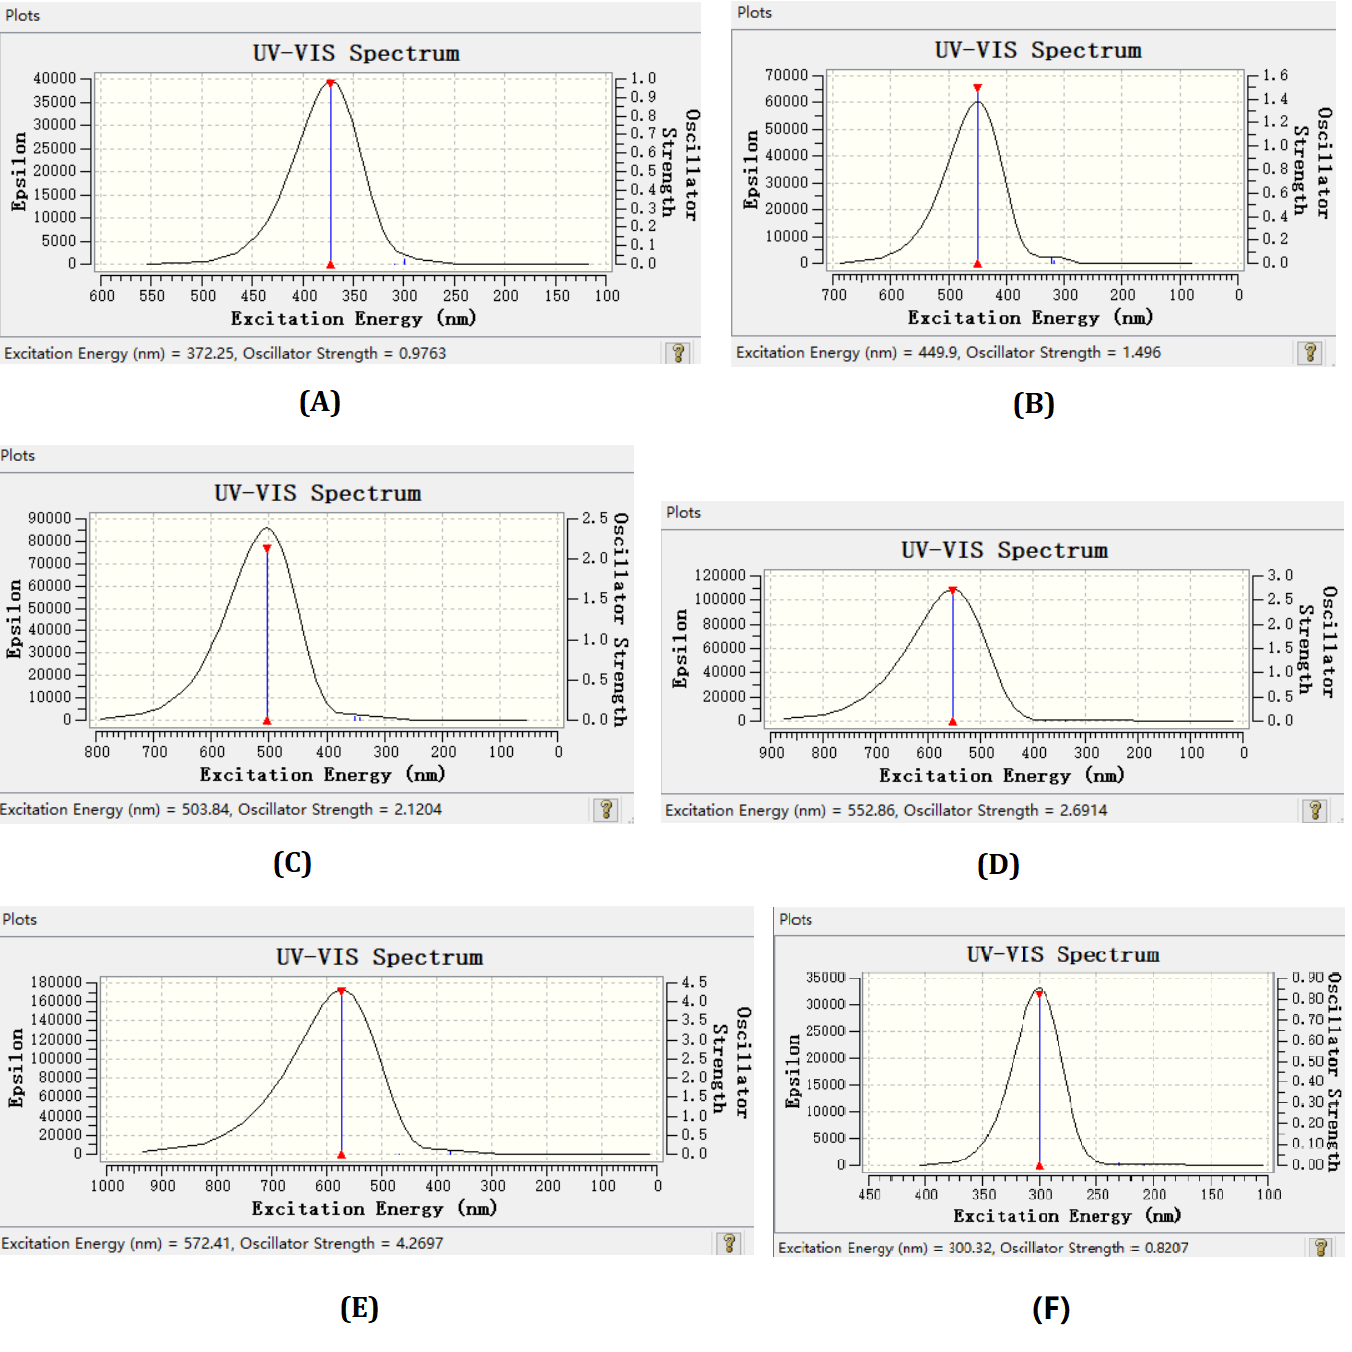
\includegraphics[width=0.8\textwidth]{7.png}
	\bicaption{Gaussian计算预测各分子的吸收光谱}{Absorption spectrum of each molecule predicted via Gaussian calculation}
\end{figure}
\par 
根据\textbf{图7},把理论计算结果与实验测得结果加以比对,计算两种方法得到的$\lambda_{max}$差值
$$\Delta\lambda_{max}=\lambda_{max, exp}-\lambda_{max, calc}
$$
结果示于\textbf{表5}。
\begin{table}[h]
	\centering
	\zihao{5}
	\bicaption{Gaussian计算与实验测得$\lambda_{max}$的比较}{Comparison of $\lambda_{max}$ obtained by Gaussian calculation and experiment}
	\begin{tabular}{cccc}
		\toprule
		分子  & $\lambda_{max, exp}/{\rm nm} $ & $\lambda_{max, calc} / {\rm nm} $& $\Delta\lambda_{max}/{\rm nm} $  \\
		\midrule
		(A) & 420.5 & 372.2 & 48.3 \\
		(B) & 555.3 & 449.9 & 105.4 \\
		(C) & 648.9 & 503.8 & 145.1 \\
		(D) & 740.2 & 552.9 & 187.3 \\
		(E) & 452.9 & 572.4 & -119.5 \\
		(F) & / & 300.3 & / \\		
		\bottomrule
	\end{tabular}
\end{table}
\par
根据\textbf{表5}可以看出,Gaussian理论计算在预测本次实验的6个分子的吸收光谱上表现不甚理想,大部分计算值与实验值有明显差别,这可能是使用Gaussian基组对复杂分子进行计算时,大量近似带来的不可忽视的误差导致的。
\subsubsection{一维势阱模型的验证}
根据一维势阱模型,长度为$L$的势阱中,量子数为$n$的电子能量为
$$E=\frac{n^{2}h^{2}}{8mL^{2}}
$$
吸收光子从$n$态跃迁到$n+1$态,光子能量等于能级差,有
$$\Delta E=\frac{(2n+1)h^{2}}{8mL^{2}}=\frac{hc}{\lambda}
$$
故预测吸收光波长
$$\lambda=\frac{8mcL^{2}}{(2n+1)h}
$$
\par 
查询\textit{Lange's Handbook of Chemistry}获得各化学键的键长数据\citealp{dean1992lange},示于\textbf{表6}。
\begin{table}[h]
	\centering
	\zihao{5}
	\bicaption{各化学键的键长数据}{Bond length data of each chemical bond}
	\begin{tabular}{ccc}
		\toprule
		化学键  & 键长$l/{\rm \AA} $ & 备注  \\
		\midrule
		\ce{C=C} & 1.336 & 共轭双键  \\
		\ce{C-C} & 1.426 & 共轭双键  \\
		\ce{C-C} & 1.395 & 芳环  \\
		\ce{C=N} & 1.320 & 共轭杂环  \\
		\ce{C-N} & 1.353 & 共轭杂环  \\
		\bottomrule
	\end{tabular}
\end{table}
\par
根据\textbf{表6}数据和\textbf{图1}各分子结构,估计一维势阱长度$L$,判断量子数$n$,用一维势阱模型计算最大吸收波长$\lambda_{max, quant}$(quant for quantum),并与实验值$\lambda_{max, exp}$对比,相关数据示于\textbf{表7}。
\begin{table}[h]
	\centering
	\zihao{5}
	\bicaption{一维势阱模型计算$\lambda_{max}$}{Calculation of $\lambda_{max}$ via one-dimensional potential well model}
		\begin{tabular}{ccccc}
			\toprule
			分子  & $\lambda_{max, exp}/{\rm nm} $ & n&$L/{\rm \AA}$ & $\lambda_{max, quant}/{\rm nm} $  \\
			\midrule
			(A) & 420.5 & 11 & 13.69 & 268.7\\
			(B) & 555.3 & 12 & 16.45 & 356.9\\
			(C) & 648.9 & 13 & 19.21 & 450.6\\
			(D) & 740.2 & 14 & 21.97 & 548.8\\
			(E) & 452.9 & 11 & 23.43 & 787.0\\
			(F) & / & 3 & 6.86 & 221.7\\	
		\bottomrule
	\end{tabular}
\end{table}
\par
\textbf{表7}计算得到的数据与实验值差异异常大,可能的原因一是势阱长度$L$的估计太过粗糙,与真实值差距极大;二是题中所提供的分子具有复杂的平面结构,用一维势阱模型计算本身就是精确度很低的。我们可以发现,对于共轭体系较小且没有苯环的分子$\rm (F)$,一维势阱模型计算的结果与查阅文献获得的实验值相对比较接近,说明一维势阱模型对于该类简单的线性共轭分子是很好的近似;而对于复杂的、具有苯环的平面共轭分子,使用一维势阱模型进行估算会造成很大误差,或者需要对势阱长度$L$进行相当精确地估计才能较好地获得近似结果。


 	 \section{讨论与结论}
		\subsection{实验讨论}
 			\subsubsection{测量吸光度的误差来源}
本次实验搭建的紫外可见分光光谱仪无法充分遮光,仅用遮光布对光谱仪进行遮罩,且每次更换样品需要翻开遮光布,环境光对于光谱仪的测量造成了一定的影响;即使在每次测量前都重测一次无样品的乙醇溶液作为参比,仍然可能由于环境光强度不同而产生一定的误差。在实际实验中,本组因为时间紧张等原因未在每次对样品测定前重测乙醇溶液作为参比,造成了严重的实验误差,因此改换溶液时重测溶剂背景是极有必要的。\par 

 	 	\subsubsection{实验改进}
 	 \subsection{实验结论}
本实验利用实验室提供的器件自主搭建了紫外可见光谱仪,利用氘灯对光谱仪进行标定,确定了$\lambda$-pixel的线性换算关系。用所搭建的光谱仪测定了同一物质不同浓度的溶液的吸收光谱,观察不同浓度下吸收光谱的差异。对比了氘灯光源和卤钨灯光源的区别,讨论了选取光源的依据。对所给的6个共轭分子的吸收光谱进行了测定,计算了各分子的摩尔消光系数$\varepsilon$。利用Gaussian程序模拟和一维势阱模型对6个共轭分子的吸收光谱或最大吸收波长$\lambda_{max}$进行了计算,比较了计算结果与实验结果的差异,探讨了差异可能的原因。
 
 

   

\vbox{}  

\bibliographystyle{achemso}
\bibliography{cite}



\end{document}